% !TeX program = pdfLaTeX
\documentclass[smallextended]{svjour3}       % onecolumn (second format)
%\documentclass[twocolumn]{svjour3}          % twocolumn
%
\smartqed  % flush right qed marks, e.g. at end of proof
%
\usepackage{amsmath}
\usepackage{graphicx}
\usepackage[utf8]{inputenc}

\usepackage[hyphens]{url} % not crucial - just used below for the URL
\usepackage{hyperref}
\providecommand{\tightlist}{%
  \setlength{\itemsep}{0pt}\setlength{\parskip}{0pt}}

%
% \usepackage{mathptmx}      % use Times fonts if available on your TeX system
%
% insert here the call for the packages your document requires
%\usepackage{latexsym}
% etc.
%
% please place your own definitions here and don't use \def but
% \newcommand{}{}
%
% Insert the name of "your journal" with
% \journalname{myjournal}
%

%% load any required packages here
\usepackage{amsfonts} \usepackage{algorithm}
\usepackage[noend]{algpseudocode}
\makeatletter \def\BState{\State\hskip-\ALG@thistlm}
\makeatother \usepackage{booktabs} \usepackage{longtable}
\usepackage{array} \usepackage{multirow} \usepackage[table]{xcolor}
\usepackage{wrapfig} \usepackage{float} \usepackage{colortbl}
\usepackage{pdflscape} \usepackage{tabu} \usepackage{threeparttable}
\usepackage{threeparttablex} \usepackage[normalem]{ulem}
\usepackage{makecell}



\begin{document}

\title{Metric space change point detection \thanks{Grants or other notes about the article that should go on the front page
should be placed here. General acknowledgments should be placed at the
end of the article.} }


    \titlerunning{Metric change point detection}

\author{  David Letscher \and  Darrin Speegle \and  }


\institute{
        David Letscher \at
     Department of Computer Science, Saint Louis University \\
     \email{\href{mailto:david.letscher@slu.edu}{\nolinkurl{david.letscher@slu.edu}}}  %  \\
%             \emph{Present address:} of F. Author  %  if needed
    \and
        Darrin Speegle \at
     Department of Mathematics and Statistics, Saint Louis University \\
     \email{\href{mailto:darrin.speegle@slu.edu}{\nolinkurl{darrin.speegle@slu.edu}}}  %  \\
%             \emph{Present address:} of F. Author  %  if needed
    \and
    }

\date{Received: date / Accepted: date}
% The correct dates will be entered by the editor


\maketitle

\begin{abstract}
Let \((x_t)_{t = 1}^N\) be a time series with values in a metric space
\(X\), which is locally isometric to Euclidean space. A transformation
of the data is proposed which produces a multi-dimensional time series
of real numbers. If the original sequence of data points has a single
change point in mean at time \(t_0\), then with high probability the
transformed data will also have a single change point in mean at time
\(t_0\). Applications to time series of persistence diagrams are
considered.
\\
\keywords{
        change point detection \and
        metric space \and
        persistence \and
        tda \and
    }

    \subclass{
                    MSC code 1 \and
                    MSC code 2 \and
            }

\end{abstract}


\def\spacingset#1{\renewcommand{\baselinestretch}%
{#1}\small\normalsize} \spacingset{1}


\section{Introduction}\label{intro}

A simple change point detection problem is the following: suppose that
\((x_t)_{t = 1}^{t_0}\) are iid Gaussian random variables with mean
\(\mu_0\) and variance \(\sigma\), and \((x_t)_{t = t_0 + 1}^N\) are iid
Gaussian with mean \(\mu_1\) and variance \(\sigma\). The goal is to
determine whether \(\mu_0 = \mu_1\), and if not, then what the value of
\(t_0\) is.

\begin{center}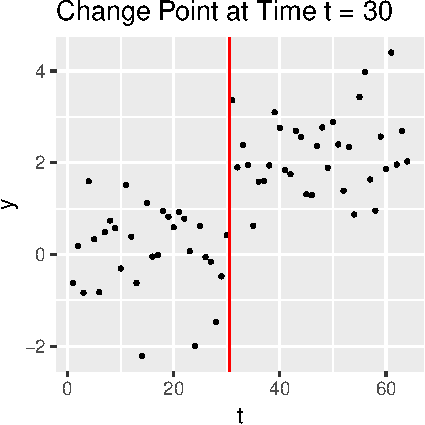
\includegraphics{springer_template_files/figure-latex/chunk_1-1} \end{center}

More general problems include having multiple change points, noise that
is not Gaussian, underlying signals that are not constant, and
multi-dimensional signals.

In this paper, we consider the following set-up. Let \(X\) be a metric
space. Supose that \(f:[0,1]\to X\) is a piecewise continuous function
with at most one discontinuity. Let \((a_t)_{t = 1}^N\) be an increasing
sequence of numbers in \((0, 1)\) and \(\delta > 0\) such that for each
\(y\in [0,1]\), \(B_\delta(f(y))\) is isometric to Euclidean space. Let
\(x_t = f(a_t) + \epsilon_t\), where \(\epsilon_t\) is a uniformly
distributed random variable on \(B_\delta(f(a_t))\). Our problem is to
determine whether there exists a point of discontinuity \(y_0\) of \(f\)
and a \(k < N\) such that the discontinuity is contained between \(a_k\)
and \(a_{k +1}\). If there does exist such a \(k\), then we should also
estimate it.

Our motivation is that we wish to find change points in time series of
\textbf{persistence diagrams}. Persistence diagrams are a way of
measuring the topological structure of a point cloud in Euclidean space.
More here.

\section{Metric space change point detection algorithm}\label{sec:1}

With the notation as set up in Section \ref{intro}, we proceed to
describe the algorithm for change point detection for time series data
in metric spaces. The main step is transforming the data into a
multi-dimensional time series of real numbers in such a way as to
preserve the change point, see Algorithm \ref{euclid}.

\begin{algorithm}
\caption{Transform to Real}\label{euclid}
\begin{algorithmic}[1]
\Procedure{MyProcedure}{}
\State $\textit{time\_length} \gets \text{length of }\textit{time\_series}$
\State $i \gets 1$
\While {$\textit{i < time\_length}$}
\State $\textit{A, B} \gets \text{sample(N, 2, replace = FALSE)}$
\For {$j \gets 1:time\_length$}
\State $\textit{dists[j,i]} \gets (d(A, x_j)^2 - d(B, x_j)^2)/d(A, B)$
\EndFor
\State $\textit{i++}$
\EndWhile
\EndProcedure
\end{algorithmic}
\end{algorithm}

Once the metric space valued time series is transformed into a
multi-dimensional real valued time series, standard techniques can be
used to determine if and where a change point occurs. In this paper, we
use the \texttt{cpbaywave} package, as it finds change points in high
dimensional, smooth data with a single discontinuity. We illustrate the
usage with some examples.

\textbackslash{}begin\{example\} Suppose that the time series lives in
\(\mathbb {R}^M\) for some \(M\). For example, we could have a time
series of length 128 in 100 dimensional data, with a change point at
time \(t = 80\). We consider two examples in this case; in both
examples, the data has mean zero in all dimensions until time 80. In the
first case, it has mean 0.1 in all dimensions from dimension 81 through
128 and in the second case it has mean 1 and all dimensions from
dimension 81 through 128.

In the case that the mean increases to 0.1, the algorithm is not able to
locate the change point, and incorrectly determines that there is no
change. In the case that the mean increases to 1, the algorithm strongly
indicates that the change point is at time \$t = 80.

\begin{center}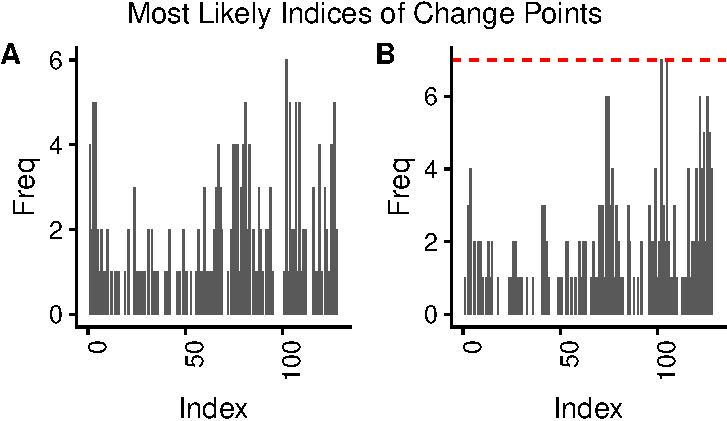
\includegraphics{springer_template_files/figure-latex/chunk_3-1} \end{center}

The following plot indicates that a change point is detected in both the
original and the transformed data at time \(t = 80\).

\begin{center}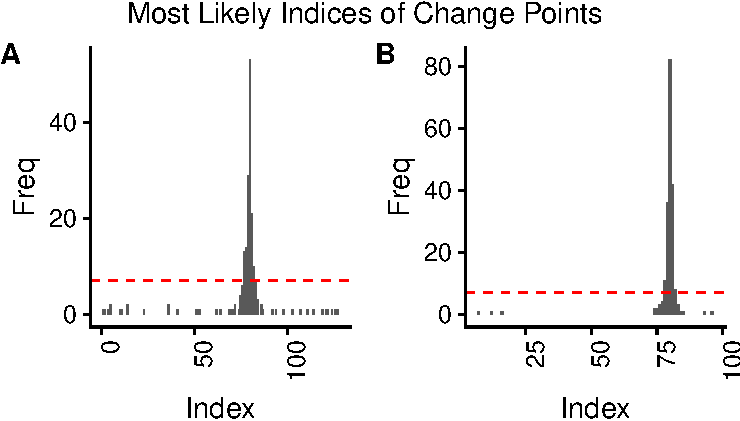
\includegraphics{springer_template_files/figure-latex/chunk_4_5-1} \end{center}

\begin{longtable}[t]{lrll}
\caption{\label{tab:chunk_4_5}Indices which are significant, together with their frequency.}\\
\toprule
\multicolumn{2}{c}{Raw Data} & \multicolumn{2}{c}{Transformed Data} \\
\cmidrule(l{2pt}r{2pt}){1-2} \cmidrule(l{2pt}r{2pt}){3-4}
Index & Freq & Index & Freq\\
\midrule
77 & 13 & 78 & 11\\
78 & 14 & 79 & 36\\
79 & 29 & 80 & 82\\
80 & 53 & 81 & 42\\
81 & 21 & 82 & 8\\
82 & 10 &  & \\
\bottomrule
\end{longtable}

This picture gives a typical strong indication that there is a change
point at or near time \(t = 80\), which we know is the correct value.

We note here that the \texttt{cpbaywave} algorithm also fails to detect
a change point in the first example when using the untransformed data.
\textbackslash{}end\{example\}

Next, we consider the same change point scenario as above, but we
imagine the time series living in \(\ell_{100}^4\) rather than in
\(\ell_{100}^2\).

\begin{center}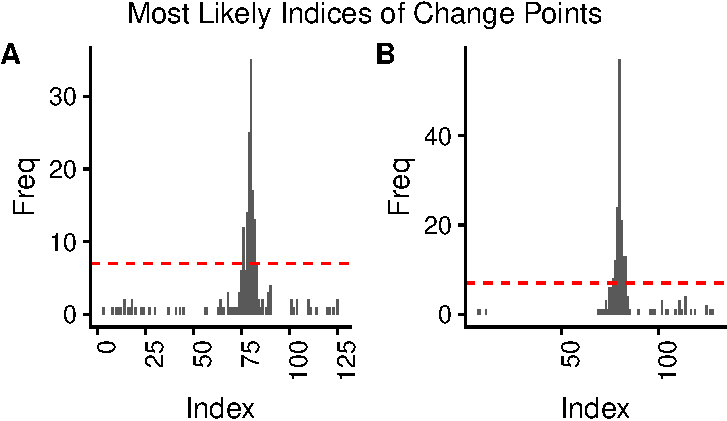
\includegraphics{springer_template_files/figure-latex/chunk_5_5-1} \end{center}

\begin{longtable}[t]{lllr}
\caption{\label{tab:chunk_5_75}Indices which are significant, together with their frequency.}\\
\toprule
\multicolumn{2}{c}{Raw Data} & \multicolumn{2}{c}{Transformed Data} \\
\cmidrule(l{2pt}r{2pt}){1-2} \cmidrule(l{2pt}r{2pt}){3-4}
Index & Freq & Index & Freq\\
\midrule
76 & 12 & 77 & 8\\
78 & 14 & 78 & 12\\
79 & 25 & 79 & 24\\
80 & 35 & 80 & 57\\
81 & 17 & 81 & 21\\
\addlinespace
82 & 13 & 82 & 13\\
 &  & 83 & 13\\
\bottomrule
\end{longtable}

The algorithm is still easily able to detect the change point at time
\(t = 80\), and in fact, does so better than the algorithm applied
directly to the unstranformed data.

\section{Change points in persistence diagrams}\label{sec:2}

The space of persistence diagrams is not locally isometric to Euclidean
space. However, it does seem to be closer to being isometric to
Euclidean space than \(\ell^4\) is. We apply our algorithm now for time
series of persistence diagrams. First, we apply it to simulated data,
then to data in the wild of various types.

Our first example is a proof of concept. We start with a single circle,
sampled randomly, and then at time \(t = 80\), we add a second disjoint
circle. Any good change point detection algorithm based on persistence
diagrams should be able to find such a change. Here are two plots of
typical point clouds in \(\mathbb{R}^2\).

\begin{center}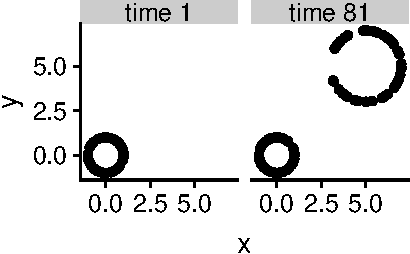
\includegraphics{springer_template_files/figure-latex/chunk_6-1} \end{center}

The change point detection algorithm easily detects the change:

\begin{center}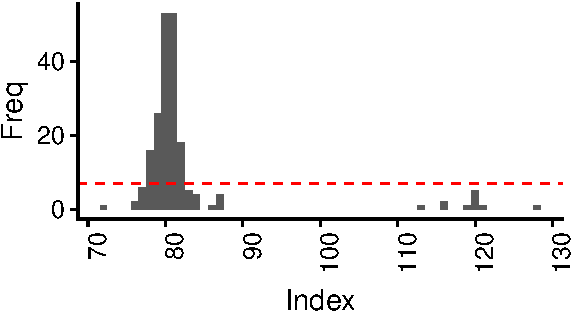
\includegraphics{springer_template_files/figure-latex/unnamed-chunk-1-1} \end{center}

\begin{longtable}[t]{lr}
\caption{\label{tab:unnamed-chunk-2}Indices which are significant, together with their frequency.}\\
\toprule
Index & Freq\\
\midrule
78 & 16\\
79 & 26\\
80 & 53\\
81 & 53\\
82 & 18\\
\bottomrule
\end{longtable}

Next, we consider two circles which start out being disjoint, but one of
the two circles passes through the other circle. From a topological
point of view, there are two potential change points. The first change
point is when there are no longer two connected components, but rather
one. The second change is when there are three loops rather than two.
The algorithm currently under discussion only finds a single change
point; how many and which dimensions are included in the persistence
diagram and distance calculation will determine which change is
detected.

Here are plots from various times in the time series.

\begin{center}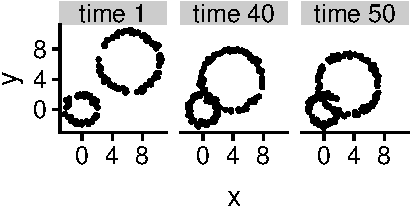
\includegraphics{springer_template_files/figure-latex/chunk_7-1} \end{center}

We see that the change point detection algorithm detects approximately
when there are three distinct loops. Note that in this case, we only
used 1-dimensional homology, so it would not be able to detect changes
in clusters.

\begin{center}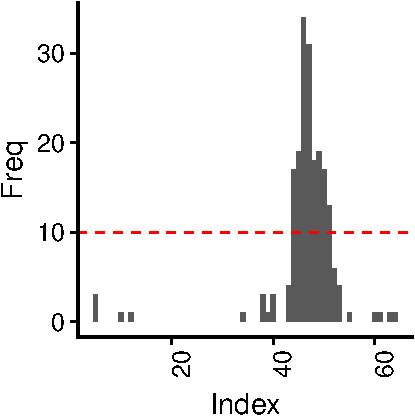
\includegraphics{springer_template_files/figure-latex/chunk_7_5-1} \end{center}

\begin{longtable}[t]{lr}
\caption{\label{tab:unnamed-chunk-3}Indices which are significant, together with their frequency.}\\
\toprule
Index & Freq\\
\midrule
44 & 17\\
45 & 19\\
46 & 34\\
47 & 31\\
48 & 18\\
\addlinespace
49 & 19\\
50 & 17\\
51 & 13\\
\bottomrule
\end{longtable}

Next, we have two examples of time series of images. In the first
example, we examine the Archive of Many Outdoor Scenes. We picked a
camera that was taking pictures of Table Mountain from Bloubergstrand in
South Africa. For each day, we averaged all of the pictures that were
taken on that day. We then used edge detection to extract edges from the
pictures, and we removed the time stamp. Finally, we randomly sampled
points from the detected edges of the pictures to use as our point
cloud. So, the time series consists of randomly sampled points from
edges of the average of all pictures on 128 consecutive days.

In the next, we have a series of images of a cell, which divides at time
\(t = 23\). We use the \texttt{cannyEdges} function in the
\texttt{imager} R package to detect the edges of the cells. We then
randomly sample 200 points from the detected edges at each time stamp to
form our time series of point clouds. We then applied the change point
detection algorithm to obtain the results below.

Here are sample images from before and after the splitting of the cell,
together with samples from the detected edges.

\begin{center}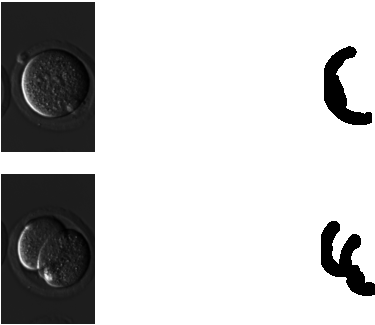
\includegraphics{springer_template_files/figure-latex/chunk_10_5-1} \end{center}

When running the algorithm, we obtain the following.

\begin{center}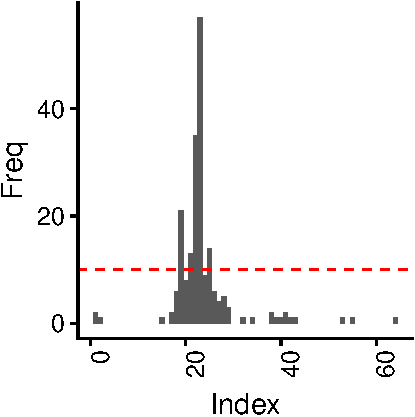
\includegraphics{springer_template_files/figure-latex/chunk_11-1} \end{center}

The significant indices from the bootstrap are:

\begin{longtable}[t]{lr}
\caption{\label{tab:chunk_12}Indices which are significant, together with their frequency.}\\
\toprule
Index & Freq\\
\midrule
19 & 21\\
21 & 13\\
22 & 35\\
23 & 57\\
25 & 14\\
\bottomrule
\end{longtable}

\section{References}\label{references}

\bibliographystyle{spbasic}
\bibliography{bibliography.bib}

\end{document}
